\subsection{Problem 15}

Find the currents in the circuit, assuming all resistances are 10 Ohm.
\begin{figure}[h]
    \centering
    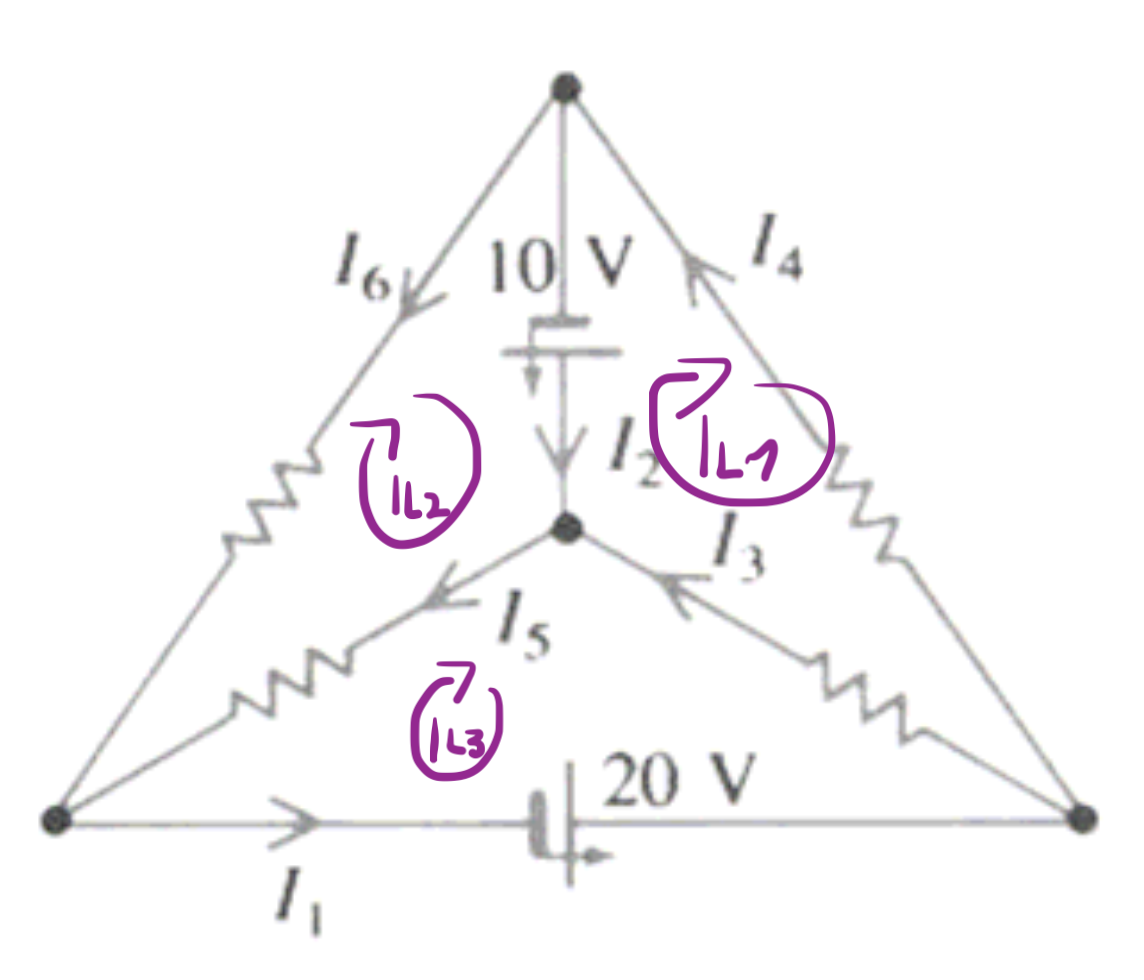
\includegraphics[width=0.5\textwidth]{images/electro.png}
    \label{fig:electro}
\end{figure}

\subsubsection*{Solution}

\begin{equation*}
    \left\{\begin{matrix}
I_{L1}(R_1 + R_2) - I_{L3}(R_2) = -E_2\\ 
I_{L2}(R_3 + R_4) - I_{L3}(R_3) = E_2\\ 
-I_{L1}(R_2) - I_{L2}(R_3) + I_{L3}(R_2 + R_3) = -E_1
\end{matrix}\right.
\end{equation*}

After substitution we have:

\begin{equation*}
    \begin{amatrix}{1}{1}
        \matr{A} & \matr{b}
    \end{amatrix} = 
    \begin{amatrix}{3}{1}
        20 & 0 & -10 & -10 \\
        0 & 20 & -10 & 10 \\
        -10 & -10 & 20 & -20
    \end{amatrix}
    \xrightarrow[magic]{}
    \begin{amatrix}{3}{1}
        1 & 0 & 0 & -1.5 \\
        0 & 1 & 0 & -0.5 \\
        0 & 0 & 1 & -2
    \end{amatrix}
\end{equation*}

\begin{equation*}
\left\{\begin{matrix}
I_1 = -I_{L3} \\
I_2 = -I_{L1} + I_{L2} \\
I_3 = I_{L1} - I_{L3} \\
I_4 = -I_{L1} \\
I_5 = I_{L2} - I_{L3} \\
I_6 = -I_{L2}
\end{matrix}\right.
\end{equation*}

\begin{equation*}
\left\{\begin{matrix}
I_1 = 2 \\
I_2 = 1 \\
I_3 = 0.5 \\
I_4 = 1.5 \\
I_5 = 1.5 \\
I_6 = 0.5
\end{matrix}\right.
\end{equation*}
